\documentclass[11pt]{article}
\usepackage[T1]{fontenc}
\usepackage[utf8]{inputenc}
\usepackage{textcomp}
\usepackage{amsmath,amssymb}
\usepackage{lmodern}
\usepackage{microtype}
\usepackage{xcolor}
\usepackage[a4paper,margin=2.4cm]{geometry}
\usepackage{longtable,booktabs,array}
\usepackage{graphicx}
\usepackage{float}
\usepackage{titletoc}
\titlecontents{section}[0pt]{\addvspace{1pt}\bfseries}{\contentslabel{1.8em}}{\hspace*{-1.8em}}{\hfill\contentspage}
\titlecontents{subsection}[1.8em]{}{\contentslabel{2.6em}}{}{\titlerule*[0.6pc]{.}\contentspage}
\usepackage{pgfplots}
\pgfplotsset{compat=1.16}
\usepackage{fancyhdr}
\usepackage[colorlinks=true,linkcolor=blue!50!black,urlcolor=blue!50!black,pdftitle={Fire Detection \& Autonomous Emergency Response},pdfauthor={Group 4: Nagarajan Ganesan (naggan-4)}]{hyperref}
\graphicspath{{../docs/diagrams/}{figures/}}
\setlength{\parindent}{0pt}\setlength{\parskip}{6pt plus 2pt minus 1pt}
\setlength{\emergencystretch}{3em}
\setcounter{secnumdepth}{2}
\providecommand{\tightlist}{\setlength{\itemsep}{0pt}\setlength{\parskip}{0pt}}
\pagestyle{fancy}\fancyhf{}
\lhead{\small Fire Detection \& Autonomous Emergency Response}
\rhead{\small D7065E\,--\,Architecture Document}
\cfoot{\thepage}
\usepackage{etoolbox}
\AtBeginEnvironment{longtable}{\footnotesize}
\newcolumntype{L}[1]{>{\raggedright\arraybackslash}p{#1}}
\AtBeginEnvironment{tabular}{\footnotesize}
\newcommand{\figH}[3]{\begin{figure}[H]\centering\includegraphics[width=#2]{#1}\caption{#3}\end{figure}}
\newcommand{\fig}[3]{\begin{figure}[htbp]\centering\includegraphics[width=#2]{#1}\caption{#3}\end{figure}}
\newcommand{\code}[1]{\texttt{#1}}

\title{Fire Detection \& Autonomous Emergency Response}
\author{D7065E Architecture Document\\[2pt] Group 4: Nagarajan Ganesan (naggan-4)}
\date{Version 1.0, 2026-10-11}

\begin{document}
\maketitle
{\small\setlength{\parskip}{0pt}\tableofcontents}
\newpage

%% ---------------------------------------------------------------- 1
\section{Summary}

\textbf{Use case.} In the course's A-building (simulated in BuildSim) the system detects a real fire, ignores false alarms such as cooking and dust, and switches on the sprinkler of the burning room. It unlocks that room's door, tells a mock emergency-responder service who is in danger and which way out is safe, and shows the route in the BuildSim 3D view while the simulated people walk out.

\textbf{Architecture.} Simulated smoke, CO and temperature sensors read a hidden physics simulation and publish their readings over an MQTT broker. A detector fuses the three signals per room with rules and a learned model (an isolation forest), and commands the sprinkler and door actuators. A responder service, a dashboard and a database writer listen to the same stream.

\textbf{Principle.} Safety comes first, then availability: a missed fire is worse than a false alarm, so a failure moves the system toward the safe action. The sprinkler still comes on when the detector or the broker is down.

\textbf{Repository:} \url{https://github.com/ennc0d3-ltu/d7065e-project}

\textbf{Changes since the proposal.} Each change has a reason.
\begin{itemize}\tightlist
\item \textbf{Data flow.} An MQTT broker feeds the detector, instead of the detector reading TimescaleDB, which put a database hop in the safety path.
\item \textbf{Services.} The proposal had a separate occupancy tracker, route planner and responder notifier. They are now one responder service: none is needed to switch on the sprinkler, they only read where people are, and they use the same inputs.
\item \textbf{Doors.} The proposal's ``unlock fire doors'' became \emph{egress} unlock, which is built: doors are locked by default, a room's door unlocks on an alarm, and the actuator fails safe. Closing doors to hold smoke back is designed but deferred.
\item \textbf{People.} The course occupancysim is used instead of our own people simulator; a small evacuation proxy makes people leave a burning room.
\item \textbf{Detector.} The learned model alone missed obvious fires (it called heavy smoke and CO ``normal'') and false-alarmed on smoke drifting in from another room. So the detector now fuses the signals two ways, a simple threshold rule and the model, and takes the higher alarm level of the two. The sprinkler also needs heat, not only smoke and CO.
\end{itemize}

%% ---------------------------------------------------------------- 2
\section{Use case and building context}

\textbf{The building.}
\begin{itemize}\tightlist
\item The course's \textbf{BuildSim}, with the embedded \emph{A-Building (LTU)} (three floors, about 970 rooms), holds the building, the devices, the sensor and actuator values, the occupancy and the 3D viewer. It simulates no physics, keeps no history, and is not modified.
\item The course also supplies \textbf{occupancysim}, which provides the people. All other components are our own: the physics simulator (Section~\ref{sec:physics}), the sensors, the detector and responder, the actuators, and the \textbf{evac-proxy}, which sits between occupancysim and BuildSim and changes only people in a room that is on fire (Section~\ref{sec:evac}).
\end{itemize}

\textbf{Actors.} The building operator monitors and may confirm, cancel or release a response; the system never requires them. Occupants do not interact with the system; they appear only as the simulated people. Emergency responders are simulated by a mock that acknowledges each dispatch.

\textbf{The scenario the demo tells.} A fire starts in the lecture hall A112\_A with about 100 people in it. The detector arms the room (the door unlocks, no water yet), then discharges the sprinkler once heat appears and persists for 15\,s. The people walk out and the responders are told (Section~\ref{sec:scenario}).

%% ---------------------------------------------------------------- 3
\section{Requirements}

Every requirement has a stable ID, a measurable criterion and a test (Section~\ref{sec:tests}). Functional requirements (FR) say what the system does and non-functional requirements (NFR) say how well. Targets marked $\dagger$ are our own starting values, to be tuned. Times are simulated seconds unless marked wall.

{\setlength{\extrarowheight}{1pt}\begin{longtable}{@{}L{1.0cm}L{0.9cm}L{5.9cm}L{5.1cm}L{1.4cm}@{}}
\toprule
ID & Prio & Requirement & Acceptance criterion & Test\\
\midrule\endhead
FR1 & Must & Each room publishes smoke, CO and temperature once per simulated second, with sequence numbers and sim-time timestamps & $\ge$ 99\% of expected messages in a fault-free run; every message has \code{seq} and \code{ts} & T1\\
FR2 & Must & The detector fuses the three signals per room into a tier (\code{none}, \code{warning}, \code{armed}, \code{fire}): a learned model with the rules as a safety floor, and a heat gate & Matches ground truth on held-out runs at the NFR2 rates; compared with the rules and the model alone & T2\\
FR3 & Must & \code{warning} and \code{armed} pre-alert; \code{fire} triggers the sprinkler, the route and the responder dispatch & Fire: sprinkler \code{on} and a dispatch. Cooking or dust: no actuator command & T3\\
FR4 & Must & Escalation by persistence, operator or both; the operator may confirm or cancel, never required & No operator input: escalates after the 15\,s persistence window. Cancel honoured for 300\,s. Every action audited & T4\\
FR5 & Must & The sprinkler latches on; only all-clear or the operator releases it & Killing the detector or dropping the score does not release it & T6\\
FR6 & Should & Egress doors locked by default; unlock for a room in alarm; unlock when the detector is silent for 30 sim s, at start-up and at shutdown. Containment closing deferred & Locked at rest, route blocked; on an alarm only that room opens; relocks when idle & T15\\
FR7 & Must & The responder service reads occupancy (read-only), classifies people as in danger, en route, safe, unaccounted for, or at risk (adjacent room), and sends a dispatch (rooms, severity, classes, routes) to the mock responder on each change and at all-clear, logging each acknowledgement & Matches the expected table for a fixed snapshot; stale occupancy shows as unknown; a dispatch with an acknowledgement for the fire, each change and the all-clear & T5\\
NFR1 & Must & Latency from the end of the 15\,s confirmation window to sprinkler \code{on}, fast and medium fires & median $\le$ 10\,s, p95 $\le$ 20\,s$^\dagger$. \textbf{Not met}, see Section~\ref{sec:quant} & T7\\
NFR2 & Must & Detector quality on 30 fire and 40 benign held-out runs & Recall $\ge$ 95\,\%; false sprinkler activation $\le$ 5\,\% (at most 2 of 40)$^\dagger$; against the baseline & T2\\
NFR3 & Must & Detector, broker or a non-core component lost: the sprinkler still comes on and the door unlocks & Detector silent for 30 sim s: actuator rules take over. Broker lost: readings arrive over the direct HTTP path. With the responder, dashboard, database writer, TimescaleDB, Grafana, Prometheus, cAdvisor and registry all stopped during a fire, the sprinkler still comes on and the door unlocks & T8, T9, T11\\
NFR4 & Must & A crashed process restarts and re-registers without manual steps & Ready and publishing within 30\,s (wall) & T10\\
NFR5 & Must & Missing, stale, duplicate and out-of-order readings are handled explicitly & Older than 15 sim s = missing and warns, never \code{normal}; duplicates dropped; gaps counted & T13\\
NFR6 & Should & Decision rounds keep up as rooms grow & 50 rooms, $10\times$ burst: round $\le$ 10\,\% of the period$^\dagger$; the limit reported & T14\\
\bottomrule
\end{longtable}}

%% ---------------------------------------------------------------- 4
\section{Architecture}

\subsection*{The system in one page}
A simulated building is watched by sensors; a detector decides whether there is a real fire; if so, the sprinkler and the room's door respond, the people walk out, and the responders are told. If any part fails, the system falls back to the safe action. Figure~\ref{fig:overview} shows the one loop that everything else supports: physics creates the fire, the sensors report it through the broker, the detector decides, an actuator acts, and BuildSim holds the new state, which the physics reads back, so the effect of the action is sensed again.

\begin{figure}[H]\centering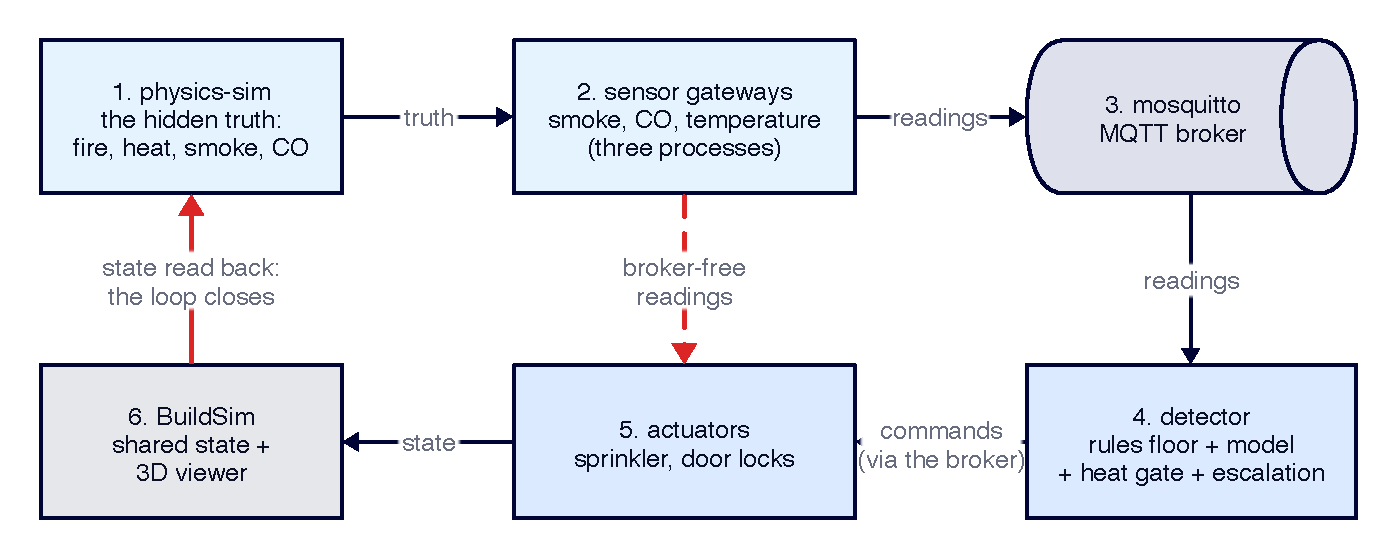
\includegraphics[width=0.8\linewidth]{overview.pdf}\caption{The sense-compute-act loop. (1)~The physics creates the fire. (2)~The sensor gateways read it, with noise and faults. (3)~The broker fans the readings out. (4)~The detector fuses them and decides. (5)~The actuators spray and unlock. (6)~BuildSim holds the new state, which the physics reads back (red, solid). The dashed red path carries readings to the actuators without the broker. Appendix~A lists every container; the C4 views follow.}\label{fig:overview}\end{figure}

The system runs as 21 containers: the simulated world (physics, BuildSim, occupancysim, evacuation proxy), the devices (three sensors, two actuators), the decision services (detector, responder), messaging and storage, and the observability and admin tools, none of which is on the safety path. Appendix~\ref{app:containers} lists each container and its job.

\subsection{Context diagram (C4 level 1)}
\fig{context.pdf}{0.8\linewidth}{C4 context: what is ours (blue) and what is outside it.}
The system talks to BuildSim (devices, state, overlays), to the course occupancysim (people, through our evacuation proxy), to the operator (a control page) and to the simulated responders (a dispatch message).

\subsection{Container diagram (C4 level 2)}
\fig{container.pdf}{0.72\linewidth}{C4 containers, part 1: the safety loop. Light blue is on the safety path, grey is course-provided or infrastructure, red is the broker-free path and the physics read-back. Appendix~\ref{app:containers} gives each container's job.}
\fig{container-people.pdf}{0.6\linewidth}{C4 containers, part 2: people and reporting, off the safety path. Dashed boxes are context.}
\fig{container-support.pdf}{0.75\linewidth}{C4 containers, part 3: supporting containers (history, dashboards, tuning, resources), off the safety path. Dashed boxes are context.}
The system is split so that each failure has a bounded effect. The control loop (gateway, broker, detector, actuator) is separate from observation and history (dashboard, db-writer, TimescaleDB, Grafana), so a crashed dashboard or database cannot stop a sprinkler. The simulator (physics) is separate from everything that would exist in a real building. Appendix~\ref{app:containers} lists every container with its job.



\subsection{Component diagram (C4 level 3): the detector}
\figH{component.pdf}{0.95\linewidth}{Inside the detector: one decision per room per period of simulated time, in six steps.}
The detector is the one container complex enough to need a component view. It makes one decision per room per period of simulated time, in six steps:
\begin{enumerate}\tightlist
\item \textbf{Service:} receives each reading and keeps the per-room state.
\item \textbf{Features:} the rolling value and slope of each signal. A failed sensor shows up as \emph{missing}, never as normal.
\item \textbf{Two classifiers} read the features: a \emph{rule baseline} (fixed thresholds; a fire needs two signals; a missing signal is at least a warning) and an \emph{anomaly model} (isolation forest).
\item \textbf{Deployed classifier:} takes the higher of the two tiers, so the model can raise a tier but never lower what the rules say. A \emph{heat gate} follows: smoke and CO alone only arm a room, and heat discharges it.
\item \textbf{Escalator:} a state machine for persistence, operator confirm and cancel, the latch until all-clear, and the audit trail.
\item \textbf{Publisher:} sends the decisions, the sprinkler and door commands and the heartbeat. History is queued during an outage; commands and heartbeats never are.
\end{enumerate}
Tuned thresholds from the registry are applied only if they stay inside the hard safety limits.

\subsection{Design decisions and alternatives}\label{sec:decisions}

{\setlength{\extrarowheight}{1pt}\begin{longtable}{@{}L{2.8cm}L{3.0cm}L{6.4cm}L{3.4cm}@{}}
\toprule
Decision & Alternatives rejected & Why (requirement) & Trade-off accepted\\
\midrule\endhead
Sensor transport: MQTT & Detector reads the database; direct REST & Several consumers need the same reading and the broker buffers for a brief outage (NFR3) & A broker to run and monitor\\
Two-tier response, rules as a floor under the model & Model alone; model with hard-limit override & Measured: the model alone rated smoke 5\,1/m and CO 500\,ppm as normal (FR2, NFR2) & False alarms are the union of both detectors\\
Smoke and CO arm, heat discharges (pre-action) & Discharge on smoke and CO; ignore smoke without heat & A room full of drifted smoke would be flooded; ignoring it leaves occupants unwarned (NFR2) & Detection is later: 110\,s against 90\,s for the model alone\\
A room that stays \emph{armed} for 120\,s escalates; a plain warning never does & Any persistent warning escalates & System test T3 showed cooking and dust discharging a sprinkler when any persistent warning escalated (NFR2, FR3) & A smoke-only smouldering fire is not escalated by persistence\\
Latch released only by all-clear & Release when the score falls & A falling score must not switch a sprinkler off during a fire (FR5) & Water runs longer than strictly needed\\
Direct gateway-to-actuator HTTP path & Second MQTT broker; NATS or Kafka; read sensors via BuildSim & A broker outage must not blind the fallback; BuildSim does not store sim time, so it cannot be the sensor source (NFR3) & One more link and a second data path\\
Outbox and dead-letter queue & Replay everything on live topics & History and dispatches survive an outage; commands and heartbeats are never replayed, because a stale command acts on a stale picture (NFR3, NFR5) & At-least-once delivery, so consumers must be idempotent\\
Course occupancysim plus an evacuation proxy & Own people simulator; fork occupancysim; overlay only & occupancysim already simulates timetables and movement; the proxy adds evacuation without changing the course code (FR7) & The proxy sits in the people feed (it fails open); evacuees do not use stairs\\
Isolation forest, one-class & Supervised fire classifier; no model & No fire data is needed for training (FR2) & Little measured benefit over the rules here\\
Hard limits on tunable thresholds & Unbounded tuning & A bad tuning run may only make the system jumpier, never blind (FR2) & Some legitimate tunings are refused\\
One container per role & One monolith & Fault isolation: a crash stays in one container and the safety loop keeps running (NFR3, NFR4) & More inter-process communication\\
\bottomrule
\end{longtable}}

%% ---------------------------------------------------------------- 5
\section{Interfaces and data contracts}

Three communication patterns are used, each for the job it fits. \textbf{MQTT} (publish/subscribe) carries readings, decisions and commands because one source feeds many consumers and the broker buffers for a briefly absent one. \textbf{REST over HTTP} carries every call to BuildSim and the small control APIs, because each is a one-to-one request whose result the caller must confirm. BuildSim's own \textbf{WebSocket} feeds its viewer.

\subsection{Messages}
Every reading carries units, a per-sensor sequence number and a sim-time timestamp, so no consumer has to guess:
\begin{verbatim}
topic sensors/level0/A1008/co          (QoS 1, not retained)
{"sensor_id":"level0-A1008-co","room":"level0/A1008","type":"co","unit":"ppm",
 "value":412.0,"seq":1873,"sim_time":418}
\end{verbatim}
A sprinkler command is idempotent and valid only for its time-to-live (sim seconds). The detector re-sends it every tick while the response is latched:
\begin{verbatim}
topic commands/sprinkler/level0/A1008  (QoS 1, never queued for replay)
{"room":"level0/A1008","action":"on","reason":"fire tier held 15s",
 "seq":14,"ttl_s":30,"sim_time":415}
\end{verbatim}

{\setlength{\extrarowheight}{1pt}\begin{longtable}{@{}L{6.6cm}L{2.2cm}L{6.8cm}@{}}
\toprule
Topic & Producer & Content and policy\\
\midrule\endhead
\code{sensors/<level>/<room>/<type>} & gateway & Reading\\
\code{decisions/<level>/<room>} & detector & Decision with its reason, and a periodic refresh\\
\code{commands/<sprinkler|door>/<level>/<room>} & detector & Sprinkler or door-unlock command with a time-to-live, re-sent every tick while in alarm. \textbf{Never queued}\\
\code{heartbeat/<process>} & every process & Liveness. \textbf{Never queued}\\
\code{dispatch/responders}, \code{dispatch/ack} & responder & Dispatch and acknowledgement. Never dropped\\
\code{dlq/<process>} & any & A message that could not be used, with the error. Never dropped\\
\bottomrule
\end{longtable}}

\subsection{HTTP endpoints}
{\setlength{\extrarowheight}{1pt}\begin{longtable}{@{}L{2.7cm}L{7.6cm}L{5.0cm}@{}}
\toprule
Process & Endpoints & Notes\\
\midrule\endhead
BuildSim (course) & under \code{/api/}: \code{PUT sensors|actuators|doors|room-layers|effects|alerts}; \code{GET occupancy|entities|graph/route} & A \code{PUT} to a collection replaces it, so each has exactly one writer. Registration repeats every 3\,s, so a BuildSim restart is repaired\\
physics-sim & \code{GET /truth/rooms/\{level\}/\{room\}}, \code{POST /control/fire|benign|clear|reset} & Truth is read only by the gateway; control is used by the scenario console\\
actuator & \code{POST /readings} & The broker-free path from the gateway\\
detector & \code{POST /operator/\{level\}/\{room\}/\{action\}}, \code{GET /status} & Operator confirm, cancel or release, all audited\\
registry & \code{GET /active}, \code{GET /bundles}, \code{POST /bundles}, \code{POST /bundles/\{v\}/promote}, \code{POST /rollback} (host port 8101) & Publishing never activates. Promotion and rollback name an approver. A bundle beyond the hard limits gets 422\\
\bottomrule
\end{longtable}}
Every process also serves \code{/healthz} and \code{/readyz}. The sensor processes accept fault injection, the evacuation proxy forwards every BuildSim call, and the scenario console forwards a fixed list of requests.

%% ---------------------------------------------------------------- 6
\section{Simulating the sensor values (the physical model)}\label{sec:physics}

BuildSim provides rooms but no physics, so our simulator (\code{physics-sim}) produces the sensor values. The model is deliberately simple. Every parameter is an assumption, and none is validated against measured fires (Section~\ref{sec:reflection}).

\textbf{Fire.} A $t^2$ growth fire (slow, medium, fast) \cite{heskestad,cfast}, with the heat release decaying exponentially once the sprinkler (state $s$) is on \cite{evans}:
\begin{equation}
Q_f(t)=\min\!\big(\alpha(t-t_0)^2,\;Q_{max}\big),\qquad
Q_{\mathrm{eff}}(t)=Q_f(t)\Big[1-s\,\big(1-e^{-(t-t_a)/\tau_{\mathrm{sup}}}\big)\Big].
\end{equation}

\textbf{Room.} One well-mixed zone per room \cite{karlsson}: a heat balance for the temperature $T$, and mass balances for smoke $K$ and CO $C$:
\begin{align}
\frac{dT}{dt}&=\frac{1}{C_{th}}\Big[k_{loss}(T_{out}-T)+q_{occ}\,n+Q_{\mathrm{eff}}-q_{spr}\,s\,(T-T_{wet})\Big]+\text{exchange},\\
\frac{dK}{dt}&=\frac{g_s Q_{\mathrm{eff}}}{V}-(\lambda_v+\lambda_s)K+\text{exchange},\qquad
\frac{dC}{dt}=\frac{g_{co} Q_{\mathrm{eff}}}{V}-\lambda_v C+\text{exchange}.
\end{align}

\textbf{Doors.} Neighbouring rooms exchange heat, smoke and CO through doors in proportion to the door openness. In the demo the rooms are isolated.

\textbf{People.} The head count $n$ comes from BuildSim's occupancy, which the course occupancysim writes (about 250 people on a weekday morning).

\textbf{Closing the loop.} The actuator writes the sprinkler state to BuildSim, and the simulator reads it back every tick, so $s$ and $t_a$ enter the equations and the room cools.

\textbf{Sensors.} A reading is the truth, delayed and degraded with Gaussian noise. Faults can be injected: stuck, offline, drift. The benign scenarios are cooking, dust, and smoke drifted from a fire elsewhere.

\textbf{Sources and assumptions.}\label{sec:sources} The forms are standard fire-science models. The parameter values (yields, mixing, time constants) are our own and are calibrated for a plausible detector response, not measured. The heat thresholds (57\,$^\circ$C, 8.3\,K/min) follow heat-detector practice \cite{heatdet}. Suppression is optimistic: Evans' time constants are hundreds of seconds \cite{evans}, ours is 60\,s. The model is not validated (ASTM E1355 was not attempted), so absolute times are not claims about real buildings. The comparisons between detectors on the same runs are the evidence.

%% ---------------------------------------------------------------- 7
\section{Autonomous services and data pipeline}\label{sec:services}

\subsection{The autonomous service}

\textbf{Inputs and outputs}
\begin{itemize}\tightlist
\item \emph{Input:} per room, every 5 sim seconds, a six-element feature vector from the last 60\,s: the latest smoke, CO and temperature, and the slope of each. A slope is trusted only once the samples span half the window.
\item \emph{Stale signals:} a signal not heard from for 15\,s is reported as missing, never read as normal.
\item \emph{Output:} a tier per room (\code{none}, \code{warning}, \code{armed}, \code{fire}), the escalator state and, while latched, a sprinkler command with a reason.
\end{itemize}

\textbf{Classification} (two detectors run on the same vector; the deployed classifier takes the higher tier)
\begin{itemize}\tightlist
\item \emph{Rule baseline:} thresholds on smoke, CO, temperature and its rate of rise. A fire needs two independent signals at fire level. With sensors failed, the confirmations shrink to the signals left, and a missing signal is at least a warning. The thresholds are checked against hard limits in code.
\item \emph{Learned model:} an isolation forest trained on normal and benign simulator data only (never a fire; the UCI occupancy dataset from the proposal is not used), with a threshold pair per sensor failure mode. Measured: with CO offline it detected 0 of 30 fires until it was calibrated per failure mode, and then all of them.
\item \emph{Heat gate:} smoke and CO at fire level without heat only \emph{arm} the room (a pre-alert, no discharge); heat discharges. If the temperature sensor is down, the gate steps aside.
\end{itemize}

\textbf{Escalation}
\begin{itemize}\tightlist
\item The fire tier must hold for 15\,s before the sprinkler discharges.
\item An armed room escalates after 120\,s (a safety valve). A plain warning never escalates alone.
\item The operator (mode \emph{both}, the default) may confirm early or cancel for 300\,s. The cancel then lapses, so a wrong cancel cannot hide a persisting fire.
\item The response stays latched until 300\,s without any signal, or an operator release.
\end{itemize}

\textbf{Why this approach.} Reacting fast to a real fire pulls one way, not flooding a room on cooking smoke or dust pulls the other, and sensors fail, lie and go silent. A single threshold cannot resolve this, so the system fuses three signals, requires heat before discharge, and keeps a deterministic floor under a learned model. The decision must also be fast, verifiable and robust to sensor failure. The course requires a learned model, so one is present, but the rules carry the safety case and the model adds little (Section~\ref{sec:eval}). The design is safe either way.

\textbf{Doors.} The rooms' doors are locked by default, so the evacuation depends on the unlock. Following fire-safety practice \cite{nfpadoor,en14637,boverket}, the detector commands an unlock as soon as a room is armed or in fire, without waiting for the sprinkler, and only for that room. The door actuator relocks when the commands stop. It unlocks everything if the detector is silent for 30 sim s, at start-up and at shutdown. Verified live. Closing containment doors is not built.

\textbf{Actuator failure behaviour}
\begin{itemize}\tightlist
\item The sprinkler actuator latches and checks each command's age and sequence.
\item If the detector is silent for 30\,s, it applies the same threshold rules to readings from MQTT \emph{and} the direct HTTP path, so it works with the broker down.
\item After a restart it adopts the state BuildSim holds, so a restart mid-fire cannot switch the sprinkler off.
\end{itemize}

\subsection{The data pipeline}
\begin{itemize}\tightlist
\item \textbf{Flow:} gateway $\to$ broker $\to$ detector, bridge and db-writer.
\item \textbf{Bridge:} writes values into BuildSim for the viewer, drops duplicates and stale messages by sequence number, counts gaps, and resets its baseline when a sender restarts.
\item \textbf{Storage:} the db-writer batches readings, decisions, commands, dispatches, dead letters and heartbeats into TimescaleDB, with sim time stored beside ingestion time. Readings are kept 7 days and the audit trail is kept. While the database is down, a bounded buffer sheds old readings before it would ever shed the audit trail.
\item \textbf{Data quality at three points:} stale signals at the detector, duplicates and gaps at the bridge, and malformed messages everywhere (counted, and set aside in a dead-letter queue). The clock between the two simulators is monitored for drift.
\item \textbf{Under failure:} a producer that cannot reach the broker writes history and dispatches to a file-backed outbox and replays them in order. Sprinkler commands and heartbeats are never queued, because replaying them would act on a stale picture. The detector re-announces each room every 30 sim s, so a consumer that missed a decision recovers.
\end{itemize}

\subsection{Tuning without weakening the detector}\label{sec:registry}
Thresholds and the model can be changed while the system runs, through a registry: a bundle is published as a candidate, a named person promotes it, and a rollback restores the previous one. Three rules keep this safe. The detector never depends on the registry (it keeps its defaults or its last good bundle). Hard limits in code refuse any bundle that makes it less sensitive than a safety limit, for example a CO fire level above 200\,ppm, so tuning can make the system jumpier but never blind. The rule floor and the heat gate are not tunable. In the demo no bundle is promoted, so the detector runs on its defaults.

\subsection{Evacuation}\label{sec:evac}
\begin{itemize}\tightlist
\item The course occupancysim has no evacuation call and is the only writer of people, so an \textbf{evacuation proxy} sits between it and BuildSim.
\item It forwards everything unchanged except people in a room the detector reports on fire. Each person reacts after 10 to 70\,s and walks the BuildSim route to the nearest safe room at 1.0 to 1.6\,m/s, so a crowd leaves over a stretch of time.
\item A route through another burning room is rejected. If every route burns, people stay.
\item The occupancy counts are rewritten in step, so the physics, the responder and the dispatch all see the room empty.
\item The responder reports each person as \emph{in danger}, \emph{en route}, \emph{safe} or \emph{unaccounted for} (in no room and not walking out). When the fire is over, people return to their timetable. If the detector cannot be reached or a body cannot be parsed, the proxy forwards unchanged.
\end{itemize}

%% ---------------------------------------------------------------- 8
\section{Behaviour}

\subsection{Key scenario (dynamic diagram)}\label{sec:scenario}
\fig{dynamic.pdf}{0.95\linewidth}{A fire, from ignition to suppression.}
\begin{itemize}\tightlist
\item \textbf{1 to 4:} the fire starts, the sensors read the truth and publish readings (3, and 3b directly to the actuators, without the broker).
\item \textbf{5:} smoke and CO arrive first and only \emph{arm} the room: a pre-alert, and the door unlocks, but no water.
\item \textbf{6 to 8:} heat plus 15\,s of persistence escalate. The detector sends the sprinkler command through the broker (the door command has been going out since the room armed).
\item \textbf{9 to 11:} the actuators write their state to BuildSim, and the physics reads it back, so the room cools: the loop closes.
\item The responder, the evacuation proxy and the dashboard work from the same decisions, off the safety path.
\end{itemize}

\subsection{Process lifecycle (state diagram)}
\fig{state.pdf}{0.95\linewidth}{The per-room escalation state machine.}
The escalator is where fault handling lives, and every transition is tested code.
\begin{itemize}\tightlist
\item A cancel is honoured for 300\,s and then lapses. A confirm reverses a cancel.
\item A cancel cannot undo a latched fire; only a release can.
\item The latch is held while the score falls, and released only by an all-clear.
\end{itemize}

%% ---------------------------------------------------------------- 9
\section{Deployment and component placement}

\fig{deployment.pdf}{0.9\linewidth}{Deployment: everything on one laptop, grouped by where each part would run in a real building.}
\begin{itemize}\tightlist
\item \textbf{One command} (\code{docker compose up}, with the course repository's path in one environment variable) builds and starts all 21 containers, including the course BuildSim and occupancysim.
\item \textbf{Loopback only:} every port is bound to the local machine, and nothing has authentication (a lab system).
\item \textbf{Restarts (NFR4):} a container healthcheck and \code{restart: unless-stopped}. The outbox lives on a volume, so a recreated container keeps its queue.
\end{itemize}

\textbf{Where computation belongs}
\begin{itemize}\tightlist
\item \emph{Edge:} the control loop (sensors, broker, detector, actuators) would run on a local edge server, so it keeps working when the internet is down.
\item \emph{Server:} the people and reporting services and everything for observation and history are off the safety path and could move to a server.
\item \emph{Simulated world:} stands in for the building. A real deployment replaces it and nothing else changes.
\end{itemize}

%% ---------------------------------------------------------------- 10
\section{Test plan}\label{sec:tests}

Unit tests run with the race detector. \emph{System} tests start the real binaries, a real broker and the real BuildSim, and then kill things. The system tests are in \code{src/systest} and are named after their ID (for example \code{TestT6\_\dots}). T7 and the recovery timings are run by \code{src/cmd/measure}, T14 by two tests in \code{internal/detectsvc}, and T2 by \code{internal/eval}. The rest are unit tests next to the code.

{\setlength{\extrarowheight}{1pt}\begin{longtable}{@{}L{1.6cm}L{6.2cm}L{1.9cm}L{5.9cm}@{}}
\toprule
ID & Test & Req. & Result\\
\midrule\endhead
T1 & Message and gap accounting for a fault-free stream & FR1 & Pass (unit tests); a full-rate run is not scripted\\
T2 & Replay held-out scenarios: rules, model, deployed & FR2, NFR2 & Section~\ref{sec:eval}\\
T3 & Fire against cooking and dust (system) & FR3 & \textbf{Pass.} Fire discharged at sim 153--158\,s; cooking and dust never (about 750 sim s)\\
T4 & Escalation modes; operator confirm and cancel & FR4 & Pass (unit tests; operator API tested)\\
T5 & Occupancy classes, dispatch, acknowledgement & FR7 & Pass (unit tests; a container run with 32 people)\\
T6 & Kill the detector during a fire & FR5 & \textbf{Pass.} Sprinkler stays on\\
T7 & 20 fires, sample-to-sprinkler latency & NFR1 & \textbf{Not met:} median 31.6\,s, p95 44.5\,s (Section~\ref{sec:quant})\\
T8 & Detector dead, then a fire & NFR3 & \textbf{Pass.} Fallback fired at sim 147\,s\\
T9, T9b & Broker dead; broker dead then back & NFR3 & \textbf{Pass.} Fire at 300\,s caught at 420\,s; 1806 outage readings replayed\\
T10, T10b & Kill each process; actuator restart mid-fire & NFR4 & \textbf{Pass.} Ready in 0.2 to 0.6\,s; sprinkler stays on\\
T11 & Responder, dashboard, database writer, TimescaleDB, Grafana, Prometheus, cAdvisor and registry stopped during a fire & NFR3 & \textbf{Pass} (run by hand, not scripted): sprinkler on, door unlocked, detector in the fire state\\
T12 & BuildSim restarts and forgets everything & NFR4 & \textbf{Pass} after a fix: registration repeats every 3\,s\\
T13 & Fire with smoke stuck, CO or temperature offline & NFR5 & \textbf{Pass.} Sprinkler on at sim 237 to 263\,s\\
T14 & Scale: rooms and burst load & NFR6 & Measured: 11\,ms per round at 5000 rooms; the broker saturates near 23\,000 readings/s\\
T15 & Doors locked at rest, unlocked on alarm, relocked when idle & FR6 & Pass (unit tests, one live check); no system test\\
\bottomrule
\end{longtable}}

%% ---------------------------------------------------------------- 11
\section{Evaluation and results}\label{sec:eval}

\textbf{Setup.} Runs use the same physics, sensor degradation and feature code as the live system, with fixed seeds. The model trains on 36 normal and benign runs (never a fire) and is tested on held-out seeds: 30 fire runs (slow, medium, fast) and 40 benign runs (normal, cooking, dust, smoke drifted from a fire elsewhere), 10 seeds each. An alarm is the fire tier held for three samples. All numbers come from simulation.

\begin{center}
\begin{tabular}{@{}lccccc@{}}
\toprule
Detector & Recall & False alarms & Alarm delay & Warning delay & Drift rooms armed\\
\midrule
Rule baseline & 1.00 & 0.00 & 110\,s & 65\,s & 1.00\\
Model alone (no heat gate) & 1.00 & 0.00$^\ast$ & 90\,s & 62\,s & 1.00\\
\textbf{Deployed} (rule floor, model, heat gate) & 1.00 & 0.00 & 110\,s & 60\,s & 1.00\\
\bottomrule
\end{tabular}
\end{center}
$^\ast$ This was 0.25 before a feature fix: the model alone false-alarmed on every drifted-smoke run. Its behaviour on drift is therefore fragile, which is why it is not trusted alone.

\textbf{How far the numbers can be trusted}
\begin{itemize}\tightlist
\item Perfect recall and zero false alarms on \emph{our own simulator} mean the benign scenarios are probably too easy (cooking stays near 0.14\,1/m, CO below 10\,ppm). The detector works here. That is not proof it is robust.
\item \textbf{The learned model adds almost nothing measurable.} With the heat gate, the deployed classifier is as fast as the rules alone (110\,s) and warns only about 5\,s earlier (within sampling noise). The delays come from sensor lag (30\,s), the persistence window (15\,s) and slow fire growth. The course requires a data-driven component, but the safety case rests on the rules.
\item Not tested: a kitchen with an oven (heat, smoke and CO all raised) trips the fixed thresholds. A model trained on that site could learn to accept it.
\end{itemize}

\subsection{Quantitative evaluation}\label{sec:quant}
The numbers come from the running stack on one laptop. Sim time runs at 10$\times$, so one real second is ten simulated seconds. Latency and recovery were measured with the tool \code{src/cmd/measure}, scale and broker throughput with two Go tests, and resources with cAdvisor. The raw output is in the repository.

\textbf{Latency (NFR1):} 20 fires (10 fast, 10 medium), all detected. Sim seconds, from the first fire-tier sample to the sprinkler on in BuildSim. Fast fires took a median of 23.2\,s and medium fires 40.7\,s, so the overall median lies between the two groups.
\begin{center}
\begin{tabular}{@{}lrr@{}}
\toprule
Segment & Median & p95\\
\midrule
First fire-tier sample $\to$ sprinkler on & \textbf{31.6\,s} & \textbf{44.5\,s}\\
Confirmation window complete $\to$ sprinkler on & 17.2\,s & 30.3\,s\\
On command $\to$ sprinkler on in BuildSim & 0.4\,s (0.04\,s wall) & 0.5\,s\\
\bottomrule
\end{tabular}
\end{center}
\begin{itemize}\tightlist
\item \textbf{NFR1 is not met}, as written or as restated. The command reaches the sprinkler in 0.04\,s of wall time, but the 15\,s confirmation window plus the 5\,s decision period already exceed the 10\,s target, and medium fires are slower (23 to 30\,s after the window) because the timer restarts whenever the tier dips near the threshold. That is the trade-off the window buys: confirmation against false discharge, paid for in response time. A shorter window was not tried.
\end{itemize}

\begin{center}
\begin{tabular}{@{}L{3.2cm}L{7.4cm}L{3.6cm}@{}}
\toprule
Measure & Result & Requirement\\
\midrule
Recovery after a kill & ready in 0.2 to 0.6\,s; first heartbeat within 2.5\,s & NFR4: met\\
Decision round & 0.1\,ms at 50 rooms, 4.3\,ms at 2000, 11\,ms at 5000 (1 to 2\,\% of the 0.5\,s budget) & NFR6: met\\
Broker throughput & saturates at about 23\,000 readings/s, 15$\times$ the load of 50 rooms & the first limit, not the detector\\
Resources & 21 containers: about 44\,\% of one core and 995\,MB; a fire changes neither & none\\
\bottomrule
\end{tabular}
\end{center}
These are laptop numbers: the production Mosquitto, the database writer and the network were not stressed.

\textbf{Defects found by evaluation and system tests} (each fixed test-first): the model missed fires with the CO sensor down and rated lethal smoke and CO as normal; a neighbouring room was flooded on drifted smoke and a kitchen discharged a sprinkler through a persistent-warning rule; a BuildSim restart and a broker outage each blinded part of the system; and start-up artefacts (a pre-alert at boot, noisy slopes) appeared only in the containerised run.

\subsection{Autonomy: how it works and how it was evaluated}\label{sec:autonomy}
\textbf{How it was evaluated.} Four kinds of evidence, each answering a different question: replay of labelled held-out runs (is the decision right?), the same replays with a sensor dead (is it right with wrong inputs?), system tests that start the real processes and kill things (does it keep working when parts fail?), and measurement of latency, recovery, scale and resources (is it fast and light enough?).
\begin{center}
\begin{tabular}{@{}L{3.3cm}L{8.3cm}L{3.4cm}@{}}
\toprule
Question & Evidence & Verdict\\
\midrule
Right decision? & Held-out runs: recall 1.00 and no false alarms; fire discharges, cooking and dust never do (system test T3) & Yes, on our own simulator\\
Right action? & Sprinkler on 0.04\,s of wall time after the command; the room's door unlocks and the route out opens (checked live) & Yes\\
Wrong inputs? & Smoke stuck, CO or temperature offline: the fire is still caught (T13) & Yes\\
Decision component down? & Detector dead, broker dead, process kills, actuator restart mid-fire, BuildSim restart (T6, T8, T9, T10, T10b, T12) & Yes\\
Independent of everything else? & Responder, dashboard, database writer, TimescaleDB, Grafana, Prometheus, cAdvisor and registry all stopped during a fire: the sprinkler still came on and the door unlocked (run by hand, not part of the automated suite) & Yes\\
Fast enough? & Median 31.6\,s from the first fire sample to sprinkler on, p95 44.5\,s, against 10\,s and 20\,s & \textbf{No}, by design: the 15\,s confirmation and the 5\,s decision period\\
\bottomrule
\end{tabular}
\end{center}
\textbf{Limits of the evidence}
\begin{itemize}\tightlist
\item The decision evidence is from our own simulator, and the benign cases are probably easy.
\item In the demo the rooms have no configured adjacency, so a fire does not spread to a neighbour and there are no at-risk rooms. Spread was exercised only offline and in system tests.
\item A wrong operator cancel is unit-tested but has no system test. The door actuator has a live check and unit tests but no system test.
\end{itemize}

\subsection{Design decisions evaluated}\label{sec:decisions-eval}
Section~\ref{sec:decisions} lists the alternatives. This table gives the verdict on the main decisions.

{\setlength{\extrarowheight}{1pt}\begin{longtable}{@{}L{3.3cm}L{1.9cm}L{5.4cm}L{4.5cm}@{}}
\toprule
Decision & Verdict & Evidence & Open limit\\
\midrule\endhead
Rule floor under the learned model & Held & Model alone called smoke 5\,1/m and CO 500\,ppm normal; deployed: recall 1.00, no false alarms & The model adds little; the same simulator is used for training and testing\\
Heat gate (smoke and CO arm, heat discharges) & Held & Cooking and dust never discharged; 10 of 10 drift runs armed & 110\,s against 90\,s without the gate; spread untested in the demo\\
15\,s confirmation window & Held, with a cost & Spikes never alarm; median 31.6\,s, p95 44.5\,s & \textbf{NFR1 not met}; a shorter window untested\\
Safety independent of the bus & Held & Sprinkler on with the detector or the broker stopped (T8, T9) & Broker and HTTP path both lost: untested; no fail-safe if the detector and all sensors fail together\\
Doors locked by default, unlocked on alarm & Held, partly tested & Live check and unit tests & No system test; a killed actuator leaves the lock state\\
Course \code{occupancysim} plus evacuation proxy & Held & 104 people classified live & No stairs or crowding\\
One container per role and sensor kind & Held & One sensor kind crashing leaves the others publishing; about 44\,\% of one core & 21 containers are harder to explain\\
\bottomrule
\end{longtable}}

%% ---------------------------------------------------------------- 12
\section{Dashboard}\label{sec:dashboard}

State and decisions are shown in three places.
\begin{itemize}\tightlist
\item \textbf{BuildSim's 3D viewer:} a fire-risk heatmap (green idle, yellow armed or warning, red fire), the evacuation route, fire, sprinkler and water effects, alert cards (critical for fire, with the reason), and a component-down alert when a heartbeat stops.
\item \textbf{Grafana} (read-only, from TimescaleDB): application health, room state over time, readings, decisions with reasons, sprinkler commands, dispatches and dead letters.
\item \textbf{Scenario console:} pick a room; set a slow, medium or fast fire, cooking or dust; clear it; act as the operator.
\end{itemize}

\begin{figure}[H]\centering
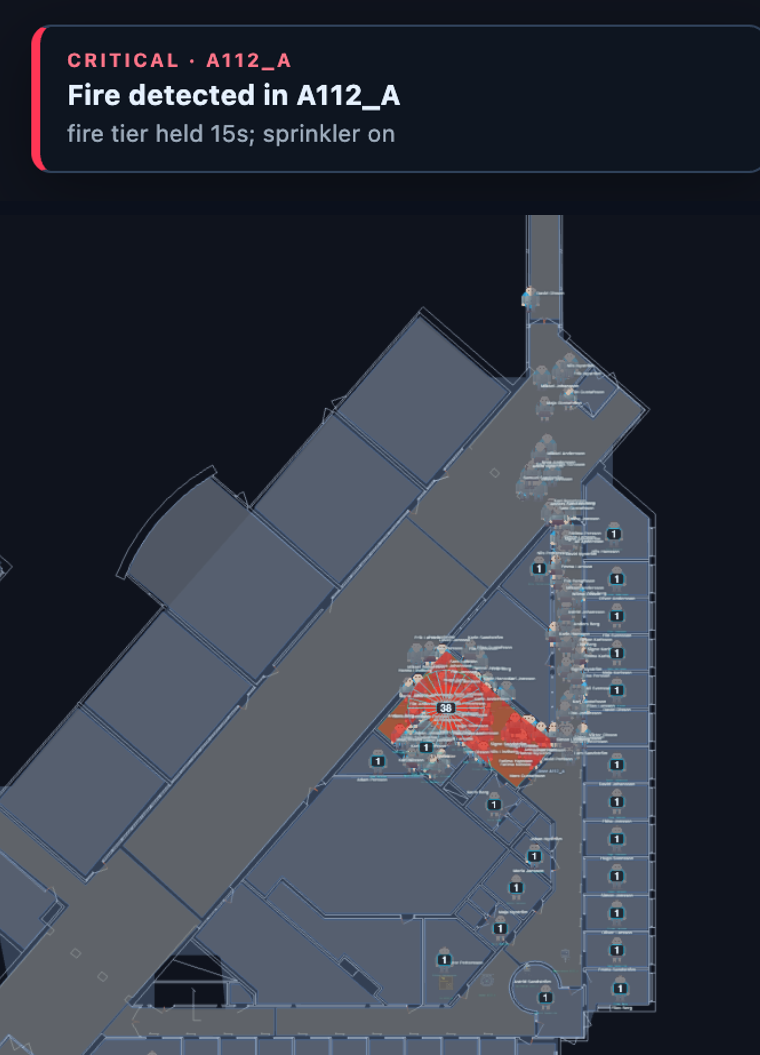
\includegraphics[width=0.35\linewidth]{viewer-fire.png}\hfill
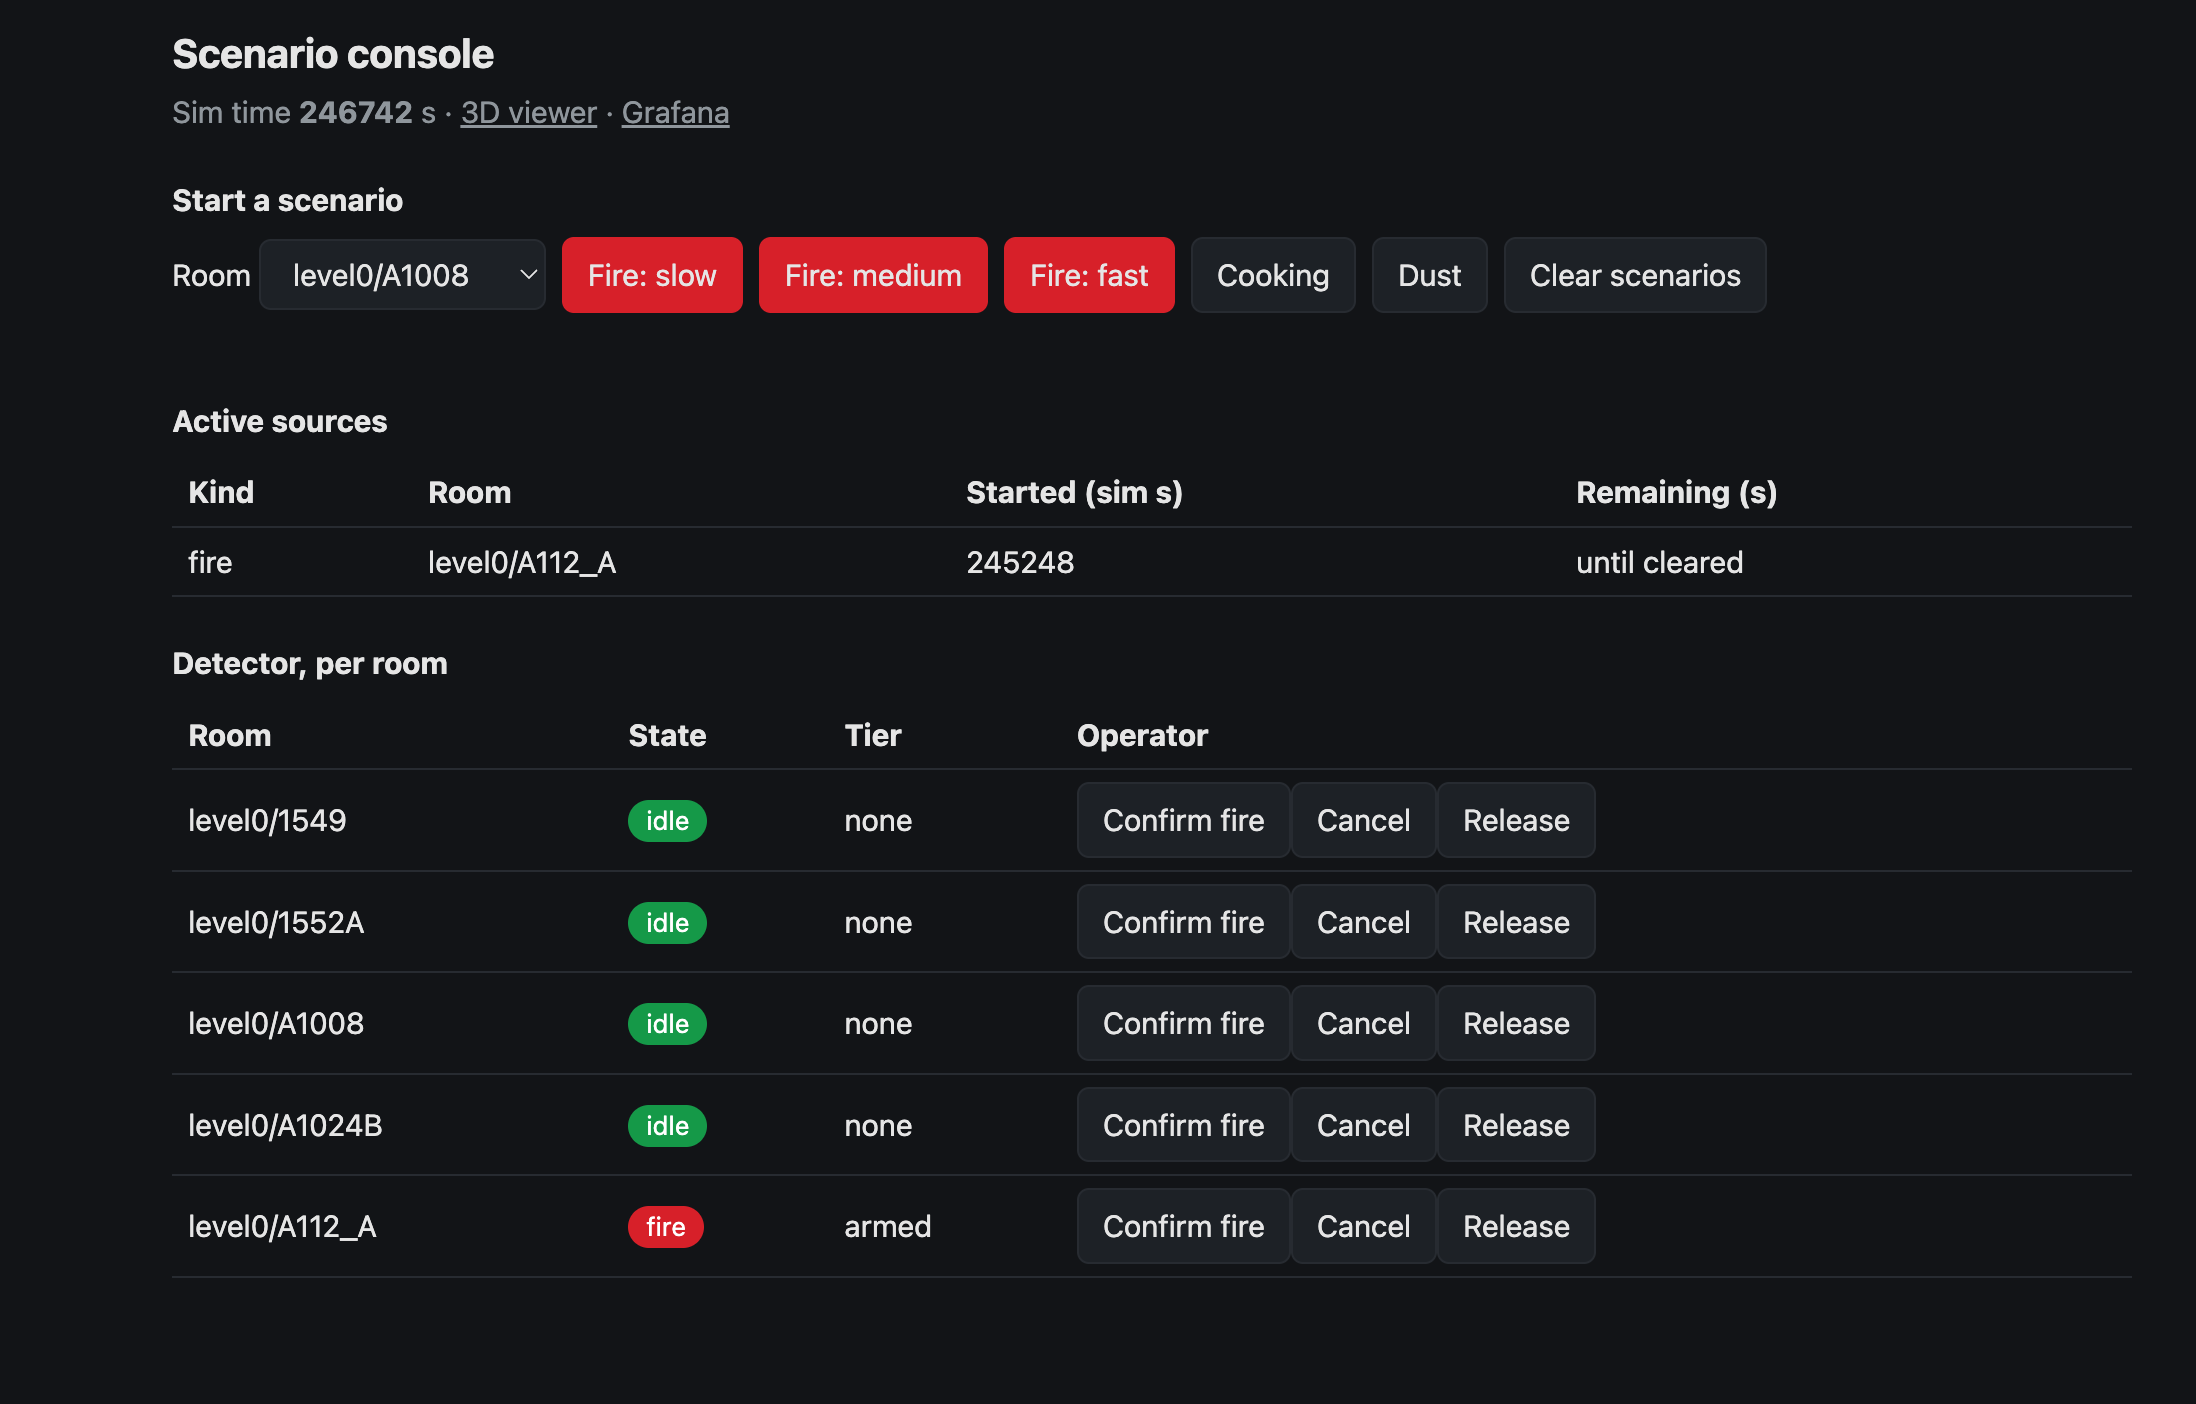
\includegraphics[width=0.61\linewidth]{scenario-console.png}
\caption{The dashboard during a fire in A112\_A. Left: BuildSim's floor plan (level 0) with the critical alert card, the red room and the people leaving along the corridor. Right: the scenario console with the active fire and the detector's state for each room.}
\end{figure}



%% ---------------------------------------------------------------- 13
\section{Risks and critical reflection}\label{sec:reflection}

\begin{itemize}\tightlist
\item \textbf{Own simulator.} Everything is tuned and evaluated on our own simulator, which is not validated against real fires, so absolute times are not claims about real buildings. The learned model's contribution is small and fragile on out-of-range inputs; the rules carry the safety case.
\item \textbf{Heat crosses an open door as freely as smoke} (one exchange coefficient). When room adjacency is configured, a neighbouring room's sprinkler therefore discharges about a minute after the source room's. Real doorways strip heat from the gas, so the model probably overstates the spread. The demo rooms are isolated, so this does not appear there.
\item \textbf{Evacuation is simple:} one route to a fixed list of safe rooms, no crowding, stairs or re-routing, and unit tests but no system test. Someone who leaves the building shows as unaccounted for. The two simulators' clocks are aligned, not locked (drift $\pm$1 to +12\,s).
\item \textbf{At-least-once messaging:} a consumer may see a message twice. Each is idempotent or deduplicates, but this is tested only for the bridge and the detector.
\item \textbf{No authentication} (the course's BuildSim design): all ports are on loopback, and any local client can call the operator API or publish sprinkler and door commands. Beyond a lab this needs TLS, per-client access lists and signed commands.
\item \textbf{Not production-ready:} the actuator's clock follows message timestamps, so if the detector and all sensors fail together no fail-safe fires; a hung container is not restarted; the broker, database and BuildSim each run once; and timeouts are in simulated seconds. A production system would use a monotonic watchdog, a clustered broker, a standby detector and synchronised clocks.
\item \textbf{Safety trade-offs:} the sprinkler stays on until a real all-clear, so water runs longer than strictly needed. If the door actuator is killed, BuildSim keeps the doors as they were until it restarts (about 0.5\,s; it also unlocks every door at start-up and shutdown). The demo locks the doors by default so that the unlock can be shown.
\item \textbf{Left out on purpose:} cold storage and cloud training, both in the proposal (the model trains in seconds on the laptop). Cost: no history beyond 7 days, and no training on real data.
\end{itemize}


\begin{thebibliography}{9}
\bibitem{heskestad} G.~Heskestad (1997), $t^2$ fire growth classes, in \emph{Fire Protection Fundamentals}, PDH Online. \url{https://pdhonline.com/courses/m282/FireProtectionFundamentals.pdf}
\bibitem{cfast} W.~W.~Jones, R.~D.~Peacock, G.~P.~Forney, P.~A.~Reneke, \emph{CFAST, Consolidated Model of Fire Growth and Smoke Transport (Version 5): Technical Reference Guide}, NIST Special Publication 1030, 2004. \url{https://nvlpubs.nist.gov/nistpubs/Legacy/SP/nistspecialpublication1030.pdf}
\bibitem{karlsson} B.~Karlsson and J.~G.~Quintiere, \emph{Enclosure Fire Dynamics}, CRC Press, 2000 (2nd ed. 2022).
\bibitem{evans} D.~D.~Evans, \emph{Sprinkler Fire Suppression Algorithm for HAZARD}, NISTIR 5254, NIST, 1993. \url{https://nvlpubs.nist.gov/nistpubs/Legacy/IR/nistir5254.pdf}
\bibitem{heatdet} System Sensor 5151 installation instructions: 135\,$^\circ$F / 57\,$^\circ$C fixed, 15\,$^\circ$F/min rate of rise; UL~521, NFPA~72. \url{https://www.manualslib.com/manual/1483746/System-Sensor-5151.html}
\bibitem{nfpadoor} DASMA, \emph{Technical Data Sheet 355: access-controlled egress doors} (NFPA 101): fail-safe on power loss, release on fire alarm or sprinkler activation. \url{https://www.dasma.com/wp-content/uploads/pubs/TechDataSheets/OperatorElectronics/TDS355.pdf}
\bibitem{en14637} EN 14637:2007, \emph{Electrically controlled hold-open systems for fire/smoke-door assemblies}. \url{https://www.sis.se/produkter/byggnadsmaterial-och-byggnader/byggnadsdelar/dorrar-och-fonster/ssen146372007/}
\bibitem{boverket} Boverket, guidance on evacuation doors and on fire and evacuation alarms (BBR chapter 7). \url{https://www.boverket.se/sv/PBL-kunskapsbanken/regler-om-byggande/brandskydd/utrymning/utrymningsdorrar/}
\end{thebibliography}

\clearpage
\appendix
\section{Container reference}\label{app:containers}
Each container in \code{docker-compose.yml} and its job. Why the system is split this way is in Sections~\ref{sec:decisions} and~\ref{sec:decisions-eval}.

\begin{longtable}{@{}L{5.4cm}L{10.2cm}@{}}
\toprule
Container & Job\\
\midrule\endhead
\code{buildsim}, \code{occupancysim} & Course-provided: the shared building state with its 3D viewer, and the people simulator\\
\code{physics-sim} & Ground truth: fire, heat, smoke and CO per room; reads the sprinkler state and the head counts back\\
\code{sensor-smoke}, \code{sensor-co}, \code{sensor-temperature} & Turn truth into degraded readings (one image, one process per kind); fault injection\\
\code{mosquitto} & MQTT broker: one reading, many consumers\\
\code{detector} & Features, model, rules, escalation, operator API\\
\code{sprinkler-actuator} & Obeys the detector, latches, local fallback\\
\code{door-actuator} & Egress door locks: locked by default, unlocked on the alarm, fails safe; the only writer of BuildSim's door collection (a \code{PUT} replaces it all)\\
\code{bridge} & Readings into BuildSim, with duplicate and gap accounting\\
\code{responder} & Danger classification and safe route; publishes the dispatch and logs the acknowledgement; read-only towards BuildSim\\
\code{dashboard} & BuildSim overlays and component health; the only writer of room layers, effects and alerts\\
\code{db-writer}, \code{timescaledb} & History and audit trail, bounded buffer\\
\code{grafana} & Application and state (read-only)\\
\code{cadvisor}, \code{prometheus} & Container CPU and memory, shown in a Grafana dashboard\\
\code{evac-proxy} & Walks people out of a burning room and keeps the occupancy counts consistent; if it fails, people stay put\\
\code{registry} & Versioned detector bundles and which one is active; the detector never depends on it\\
\code{scenario-console} & Start a fire, cooking or dust; operator buttons\\
\bottomrule
\end{longtable}


\end{document}
